% Options for packages loaded elsewhere
\PassOptionsToPackage{unicode}{hyperref}
\PassOptionsToPackage{hyphens}{url}
\documentclass[
]{article}
\usepackage{xcolor}
\usepackage[margin=1in]{geometry}
\usepackage{amsmath,amssymb}
\setcounter{secnumdepth}{-\maxdimen} % remove section numbering
\usepackage{iftex}
\ifPDFTeX
  \usepackage[T1]{fontenc}
  \usepackage[utf8]{inputenc}
  \usepackage{textcomp} % provide euro and other symbols
\else % if luatex or xetex
  \usepackage{unicode-math} % this also loads fontspec
  \defaultfontfeatures{Scale=MatchLowercase}
  \defaultfontfeatures[\rmfamily]{Ligatures=TeX,Scale=1}
\fi
\usepackage{lmodern}
\ifPDFTeX\else
  % xetex/luatex font selection
\fi
% Use upquote if available, for straight quotes in verbatim environments
\IfFileExists{upquote.sty}{\usepackage{upquote}}{}
\IfFileExists{microtype.sty}{% use microtype if available
  \usepackage[]{microtype}
  \UseMicrotypeSet[protrusion]{basicmath} % disable protrusion for tt fonts
}{}
\makeatletter
\@ifundefined{KOMAClassName}{% if non-KOMA class
  \IfFileExists{parskip.sty}{%
    \usepackage{parskip}
  }{% else
    \setlength{\parindent}{0pt}
    \setlength{\parskip}{6pt plus 2pt minus 1pt}}
}{% if KOMA class
  \KOMAoptions{parskip=half}}
\makeatother
\usepackage{color}
\usepackage{fancyvrb}
\newcommand{\VerbBar}{|}
\newcommand{\VERB}{\Verb[commandchars=\\\{\}]}
\DefineVerbatimEnvironment{Highlighting}{Verbatim}{commandchars=\\\{\}}
% Add ',fontsize=\small' for more characters per line
\usepackage{framed}
\definecolor{shadecolor}{RGB}{248,248,248}
\newenvironment{Shaded}{\begin{snugshade}}{\end{snugshade}}
\newcommand{\AlertTok}[1]{\textcolor[rgb]{0.94,0.16,0.16}{#1}}
\newcommand{\AnnotationTok}[1]{\textcolor[rgb]{0.56,0.35,0.01}{\textbf{\textit{#1}}}}
\newcommand{\AttributeTok}[1]{\textcolor[rgb]{0.13,0.29,0.53}{#1}}
\newcommand{\BaseNTok}[1]{\textcolor[rgb]{0.00,0.00,0.81}{#1}}
\newcommand{\BuiltInTok}[1]{#1}
\newcommand{\CharTok}[1]{\textcolor[rgb]{0.31,0.60,0.02}{#1}}
\newcommand{\CommentTok}[1]{\textcolor[rgb]{0.56,0.35,0.01}{\textit{#1}}}
\newcommand{\CommentVarTok}[1]{\textcolor[rgb]{0.56,0.35,0.01}{\textbf{\textit{#1}}}}
\newcommand{\ConstantTok}[1]{\textcolor[rgb]{0.56,0.35,0.01}{#1}}
\newcommand{\ControlFlowTok}[1]{\textcolor[rgb]{0.13,0.29,0.53}{\textbf{#1}}}
\newcommand{\DataTypeTok}[1]{\textcolor[rgb]{0.13,0.29,0.53}{#1}}
\newcommand{\DecValTok}[1]{\textcolor[rgb]{0.00,0.00,0.81}{#1}}
\newcommand{\DocumentationTok}[1]{\textcolor[rgb]{0.56,0.35,0.01}{\textbf{\textit{#1}}}}
\newcommand{\ErrorTok}[1]{\textcolor[rgb]{0.64,0.00,0.00}{\textbf{#1}}}
\newcommand{\ExtensionTok}[1]{#1}
\newcommand{\FloatTok}[1]{\textcolor[rgb]{0.00,0.00,0.81}{#1}}
\newcommand{\FunctionTok}[1]{\textcolor[rgb]{0.13,0.29,0.53}{\textbf{#1}}}
\newcommand{\ImportTok}[1]{#1}
\newcommand{\InformationTok}[1]{\textcolor[rgb]{0.56,0.35,0.01}{\textbf{\textit{#1}}}}
\newcommand{\KeywordTok}[1]{\textcolor[rgb]{0.13,0.29,0.53}{\textbf{#1}}}
\newcommand{\NormalTok}[1]{#1}
\newcommand{\OperatorTok}[1]{\textcolor[rgb]{0.81,0.36,0.00}{\textbf{#1}}}
\newcommand{\OtherTok}[1]{\textcolor[rgb]{0.56,0.35,0.01}{#1}}
\newcommand{\PreprocessorTok}[1]{\textcolor[rgb]{0.56,0.35,0.01}{\textit{#1}}}
\newcommand{\RegionMarkerTok}[1]{#1}
\newcommand{\SpecialCharTok}[1]{\textcolor[rgb]{0.81,0.36,0.00}{\textbf{#1}}}
\newcommand{\SpecialStringTok}[1]{\textcolor[rgb]{0.31,0.60,0.02}{#1}}
\newcommand{\StringTok}[1]{\textcolor[rgb]{0.31,0.60,0.02}{#1}}
\newcommand{\VariableTok}[1]{\textcolor[rgb]{0.00,0.00,0.00}{#1}}
\newcommand{\VerbatimStringTok}[1]{\textcolor[rgb]{0.31,0.60,0.02}{#1}}
\newcommand{\WarningTok}[1]{\textcolor[rgb]{0.56,0.35,0.01}{\textbf{\textit{#1}}}}
\usepackage{longtable,booktabs,array}
\usepackage{calc} % for calculating minipage widths
% Correct order of tables after \paragraph or \subparagraph
\usepackage{etoolbox}
\makeatletter
\patchcmd\longtable{\par}{\if@noskipsec\mbox{}\fi\par}{}{}
\makeatother
% Allow footnotes in longtable head/foot
\IfFileExists{footnotehyper.sty}{\usepackage{footnotehyper}}{\usepackage{footnote}}
\makesavenoteenv{longtable}
\usepackage{graphicx}
\makeatletter
\newsavebox\pandoc@box
\newcommand*\pandocbounded[1]{% scales image to fit in text height/width
  \sbox\pandoc@box{#1}%
  \Gscale@div\@tempa{\textheight}{\dimexpr\ht\pandoc@box+\dp\pandoc@box\relax}%
  \Gscale@div\@tempb{\linewidth}{\wd\pandoc@box}%
  \ifdim\@tempb\p@<\@tempa\p@\let\@tempa\@tempb\fi% select the smaller of both
  \ifdim\@tempa\p@<\p@\scalebox{\@tempa}{\usebox\pandoc@box}%
  \else\usebox{\pandoc@box}%
  \fi%
}
% Set default figure placement to htbp
\def\fps@figure{htbp}
\makeatother
\setlength{\emergencystretch}{3em} % prevent overfull lines
\providecommand{\tightlist}{%
  \setlength{\itemsep}{0pt}\setlength{\parskip}{0pt}}
\usepackage{bookmark}
\IfFileExists{xurl.sty}{\usepackage{xurl}}{} % add URL line breaks if available
\urlstyle{same}
\hypersetup{
  pdftitle={RNA-seq Differential Gene Expression with DESeq2},
  pdfauthor={Mery Touceda-Suárez},
  hidelinks,
  pdfcreator={LaTeX via pandoc}}

\title{RNA-seq Differential Gene Expression with DESeq2}
\usepackage{etoolbox}
\makeatletter
\providecommand{\subtitle}[1]{% add subtitle to \maketitle
  \apptocmd{\@title}{\par {\large #1 \par}}{}{}
}
\makeatother
\subtitle{UCD Bioinformatics Summer Course --- Week 2, Day 4}
\author{Mery Touceda-Suárez}
\date{2026-05-21}

\begin{document}
\maketitle

{
\setcounter{tocdepth}{3}
\tableofcontents
}
\begin{center}\rule{0.5\linewidth}{0.5pt}\end{center}

\section{Overview}\label{overview}

In this session we will take a \textbf{raw gene count matrix} from an
RNA-seq experiment and walk through a complete differential gene
expression (DGE) analysis using \textbf{DESeq2}. By the end you should
be able to:

\begin{itemize}
\tightlist
\item
  Understand what a count matrix is and why we need special statistical
  methods for it
\item
  Run a DESeq2 analysis from start to finish
\item
  Produce and interpret a PCA plot, MA plot, volcano plot, and heatmap
\item
  Extract lists of differentially expressed genes (DEGs)
\end{itemize}

\subsection{The experiment}\label{the-experiment}

We have RNA-seq data from cells sampled at \textbf{three time points}:

\begin{longtable}[]{@{}ll@{}}
\toprule\noalign{}
Label & Meaning \\
\midrule\noalign{}
\endhead
\bottomrule\noalign{}
\endlastfoot
D0 & Day 0 (baseline) \\
D7 & Day 7 \\
D14 & Day 14 \\
\end{longtable}

There are \textbf{3 biological replicates per time point} (9 samples
total). We want to find genes that change in expression over time,
comparing D7 and D14 each back to the D0 baseline.

\begin{center}\rule{0.5\linewidth}{0.5pt}\end{center}

\section{Setup}\label{setup}

\subsection{Load libraries}\label{load-libraries}

\begin{Shaded}
\begin{Highlighting}[]
\CommentTok{\# BiocManager::install("DESeq2", force = TRUE)  \# run once if not installed}
\FunctionTok{library}\NormalTok{(DESeq2)     }\CommentTok{\# core DGE analysis}
\FunctionTok{library}\NormalTok{(tidyverse)  }\CommentTok{\# data wrangling \& ggplot2}
\FunctionTok{library}\NormalTok{(pheatmap)   }\CommentTok{\# heatmap plotting}
\end{Highlighting}
\end{Shaded}

\begin{quote}
\textbf{Why these packages?}\\
\texttt{DESeq2} is a Bioconductor package specifically designed for
count-based RNA-seq data. It handles the statistical challenges of read
counts (discrete values, overdispersion, varying library sizes) better
than approaches designed for continuous data like microarrays.
\end{quote}

\begin{center}\rule{0.5\linewidth}{0.5pt}\end{center}

\section{Read in Data}\label{read-in-data}

\begin{Shaded}
\begin{Highlighting}[]
\CommentTok{\# Gene count matrix: rows = genes, columns = samples}
\NormalTok{Gene\_matrix }\OtherTok{\textless{}{-}} \FunctionTok{read.table}\NormalTok{(}\StringTok{"Gene\_matrix.txt"}\NormalTok{, }\AttributeTok{sep =} \StringTok{"}\SpecialCharTok{\textbackslash{}t}\StringTok{"}\NormalTok{, }\AttributeTok{header =} \ConstantTok{TRUE}\NormalTok{)}
\FunctionTok{dim}\NormalTok{(Gene\_matrix)}
\end{Highlighting}
\end{Shaded}

\begin{verbatim}
## [1] 28524     9
\end{verbatim}

\begin{Shaded}
\begin{Highlighting}[]
\CommentTok{\# [1] 28524     9}
\end{Highlighting}
\end{Shaded}

The count matrix contains \textbf{28,524 genes} across \textbf{9
samples}. Each value represents the number of sequencing reads that
mapped to that gene in that sample --- a proxy for how much that gene is
being expressed.

\begin{Shaded}
\begin{Highlighting}[]
\CommentTok{\# Metadata / phenotype table: one row per sample}
\NormalTok{pheno\_data }\OtherTok{\textless{}{-}} \FunctionTok{read.table}\NormalTok{(}\StringTok{"Metadata.txt"}\NormalTok{, }\AttributeTok{sep =} \StringTok{"}\SpecialCharTok{\textbackslash{}t}\StringTok{"}\NormalTok{, }\AttributeTok{header =} \ConstantTok{TRUE}\NormalTok{) }\SpecialCharTok{\%\textgreater{}\%}
  \FunctionTok{mutate}\NormalTok{(}\AttributeTok{Day =} \FunctionTok{factor}\NormalTok{(Day)) }\SpecialCharTok{\%\textgreater{}\%}              \CommentTok{\# treat Day as a categorical variable}
  \FunctionTok{column\_to\_rownames}\NormalTok{(}\StringTok{"Sample\_ID"}\NormalTok{) }\SpecialCharTok{\%\textgreater{}\%}
  \FunctionTok{mutate}\NormalTok{(}\AttributeTok{Sample\_ID =} \FunctionTok{rownames}\NormalTok{(.))}

\FunctionTok{dim}\NormalTok{(pheno\_data)}
\end{Highlighting}
\end{Shaded}

\begin{verbatim}
## [1] 9 3
\end{verbatim}

\begin{Shaded}
\begin{Highlighting}[]
\CommentTok{\# [1] 9 3}

\FunctionTok{levels}\NormalTok{(pheno\_data}\SpecialCharTok{$}\NormalTok{Day)}
\end{Highlighting}
\end{Shaded}

\begin{verbatim}
## [1] "D0"  "D14" "D7"
\end{verbatim}

\begin{Shaded}
\begin{Highlighting}[]
\CommentTok{\# [1] "D0"  "D14" "D7"}
\end{Highlighting}
\end{Shaded}

\begin{quote}
\textbf{Why \texttt{factor(Day)}?}\\
R needs to know that D0, D7, D14 are \emph{groups}, not numbers. Making
it a factor also lets DESeq2 automatically set the first alphabetical
level (D0) as the reference for comparisons --- which is exactly what we
want.
\end{quote}

\begin{Shaded}
\begin{Highlighting}[]
\CommentTok{\# CRITICAL: sample order in metadata must match column order in count matrix}
\FunctionTok{all}\NormalTok{(}\FunctionTok{rownames}\NormalTok{(pheno\_data) }\SpecialCharTok{==} \FunctionTok{colnames}\NormalTok{(Gene\_matrix))}
\end{Highlighting}
\end{Shaded}

\begin{verbatim}
## [1] TRUE
\end{verbatim}

\begin{Shaded}
\begin{Highlighting}[]
\CommentTok{\# [1] TRUE}
\end{Highlighting}
\end{Shaded}

\begin{quote}
⚠️ \textbf{This check is essential.} If the samples are mismatched, your
results will be nonsense. Always verify before running DESeq2.
\end{quote}

\begin{center}\rule{0.5\linewidth}{0.5pt}\end{center}

\section{DESeq2 Analysis}\label{deseq2-analysis}

\subsection{Build the DESeqDataSet
object}\label{build-the-deseqdataset-object}

\begin{Shaded}
\begin{Highlighting}[]
\CommentTok{\# DESeqDataSetFromMatrix needs an integer matrix + metadata + experimental design}
\NormalTok{dds }\OtherTok{\textless{}{-}} \FunctionTok{DESeqDataSetFromMatrix}\NormalTok{(Gene\_matrix, pheno\_data, }\AttributeTok{design =} \SpecialCharTok{\textasciitilde{}}\NormalTok{ Day)}
\end{Highlighting}
\end{Shaded}

The \texttt{design\ =\ \textasciitilde{}\ Day} formula tells DESeq2
which variable to use when testing for differential expression. This is
where you'd add batch effects or covariates if you had them (e.g.,
\texttt{\textasciitilde{}\ Batch\ +\ Day}).

\subsection{Filter low-count genes}\label{filter-low-count-genes}

\begin{Shaded}
\begin{Highlighting}[]
\CommentTok{\# Keep genes with at least 10 counts in at least 3 samples (our smallest group size)}
\NormalTok{smallestGroupSize }\OtherTok{\textless{}{-}} \DecValTok{3}
\NormalTok{keep }\OtherTok{\textless{}{-}} \FunctionTok{rowSums}\NormalTok{(}\FunctionTok{counts}\NormalTok{(dds) }\SpecialCharTok{\textgreater{}=} \DecValTok{10}\NormalTok{) }\SpecialCharTok{\textgreater{}=}\NormalTok{ smallestGroupSize}
\NormalTok{dds  }\OtherTok{\textless{}{-}}\NormalTok{ dds[keep, ]}

\FunctionTok{dim}\NormalTok{(dds)}
\end{Highlighting}
\end{Shaded}

\begin{verbatim}
## [1] 15922     9
\end{verbatim}

\begin{Shaded}
\begin{Highlighting}[]
\CommentTok{\# [1] 15922     9}
\end{Highlighting}
\end{Shaded}

We go from \textasciitilde28,500 genes down to
\textbf{\textasciitilde15,900} after filtering. Genes with very low
counts across all samples:

\begin{itemize}
\tightlist
\item
  Carry little statistical power (you can't reliably detect changes in a
  gene with 0--2 reads)
\item
  Increase the multiple-testing burden, raising your false-discovery
  rate
\item
  Are often noise (mapping artefacts, pseudogenes, etc.)
\end{itemize}

\subsection{Run DESeq2}\label{run-deseq2}

\begin{Shaded}
\begin{Highlighting}[]
\NormalTok{dds }\OtherTok{\textless{}{-}} \FunctionTok{DESeq}\NormalTok{(dds)}
\end{Highlighting}
\end{Shaded}

\texttt{DESeq()} does three things in one call:

\begin{enumerate}
\def\labelenumi{\arabic{enumi}.}
\tightlist
\item
  \textbf{Estimates size factors} --- normalises for differences in
  sequencing depth between samples (similar in spirit to CPM
  normalisation, but more robust)
\item
  \textbf{Estimates dispersion} --- models gene-by-gene variability.
  RNA-seq counts are overdispersed (variance \textgreater{} mean), so
  DESeq2 fits a negative binomial model rather than a simpler Poisson
  model
\item
  \textbf{Fits the GLM and tests} --- for each gene, fits a generalised
  linear model and performs a Wald test for each contrast
\end{enumerate}

\begin{center}\rule{0.5\linewidth}{0.5pt}\end{center}

\section{PCA Plot}\label{pca-plot}

Principal Component Analysis (PCA) is a quality-control step we do
\emph{before} looking at individual gene results. It reduces the entire
transcriptome to a 2D summary so we can check whether samples cluster as
expected.

\subsection{Variance-stabilising transformation
(VST)}\label{variance-stabilising-transformation-vst}

\begin{Shaded}
\begin{Highlighting}[]
\CommentTok{\# VST makes count data more suitable for PCA / clustering}
\NormalTok{vsd }\OtherTok{\textless{}{-}} \FunctionTok{vst}\NormalTok{(dds, }\AttributeTok{blind =} \ConstantTok{FALSE}\NormalTok{)}
\end{Highlighting}
\end{Shaded}

Raw counts are not suitable for PCA because highly expressed genes
dominate simply by having larger absolute variance. The VST compresses
the dynamic range so that all genes contribute more equally.
\texttt{blind\ =\ FALSE} means it uses the experimental design when
estimating dispersion --- appropriate when you're not doing blind QC.

\subsection{Create the PCA plot}\label{create-the-pca-plot}

\begin{Shaded}
\begin{Highlighting}[]
\NormalTok{pcaData   }\OtherTok{\textless{}{-}} \FunctionTok{plotPCA}\NormalTok{(vsd, }\AttributeTok{intgroup =} \StringTok{"Day"}\NormalTok{, }\AttributeTok{returnData =} \ConstantTok{TRUE}\NormalTok{)}
\NormalTok{percentVar }\OtherTok{\textless{}{-}} \FunctionTok{round}\NormalTok{(}\DecValTok{100} \SpecialCharTok{*} \FunctionTok{attr}\NormalTok{(pcaData, }\StringTok{"percentVar"}\NormalTok{))}

\NormalTok{pcaPlot }\OtherTok{\textless{}{-}} \FunctionTok{ggplot}\NormalTok{(pcaData, }\FunctionTok{aes}\NormalTok{(}\AttributeTok{x =}\NormalTok{ PC1, }\AttributeTok{y =}\NormalTok{ PC2, }\AttributeTok{color =}\NormalTok{ Day)) }\SpecialCharTok{+}
  \FunctionTok{geom\_point}\NormalTok{(}\AttributeTok{size =} \DecValTok{3}\NormalTok{) }\SpecialCharTok{+}
  \FunctionTok{xlab}\NormalTok{(}\FunctionTok{paste0}\NormalTok{(}\StringTok{"PC1: "}\NormalTok{, percentVar[}\DecValTok{1}\NormalTok{], }\StringTok{"\% variance"}\NormalTok{)) }\SpecialCharTok{+}
  \FunctionTok{ylab}\NormalTok{(}\FunctionTok{paste0}\NormalTok{(}\StringTok{"PC2: "}\NormalTok{, percentVar[}\DecValTok{2}\NormalTok{], }\StringTok{"\% variance"}\NormalTok{)) }\SpecialCharTok{+}
  \FunctionTok{coord\_fixed}\NormalTok{()}

\NormalTok{pcaPlot}
\end{Highlighting}
\end{Shaded}

\pandocbounded{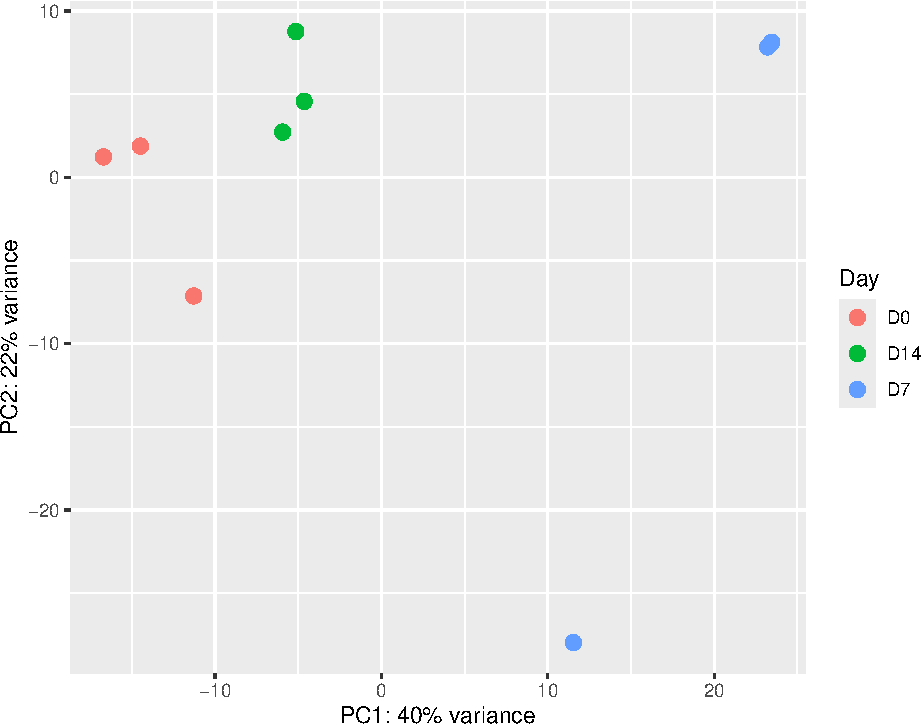
\includegraphics[keepaspectratio]{DESeq2_RNAseq_tutorial_files/figure-latex/pca-plot-1.pdf}}

\begin{Shaded}
\begin{Highlighting}[]
\FunctionTok{ggsave}\NormalTok{(}\StringTok{"PCA\_plot.pdf"}\NormalTok{, pcaPlot, }\AttributeTok{device =} \StringTok{"pdf"}\NormalTok{)}
\end{Highlighting}
\end{Shaded}

\subsubsection{How to interpret the PCA
plot}\label{how-to-interpret-the-pca-plot}

\begin{itemize}
\tightlist
\item
  \textbf{Each point is one sample.} Points close together have similar
  overall gene expression profiles.
\item
  \textbf{Good signs:} Replicates of the same time point cluster tightly
  together; different time points separate from each other. This
  confirms that Day is the dominant source of variation and that the
  experiment worked.
\item
  \textbf{Warning signs:} An outlier replicate sitting far from its
  group, or samples clustering by batch/run date rather than by Day ---
  these would need investigation before trusting DGE results.
\item
  \textbf{Variance explained:} The axis labels tell you how much of the
  total transcriptome-wide variation each PC captures. A high PC1 \%
  (e.g., \textgreater50\%) with clear group separation is a reassuring
  sign.
\end{itemize}

\begin{center}\rule{0.5\linewidth}{0.5pt}\end{center}

\section{Differential Expression
Results}\label{differential-expression-results}

\subsection{Extract results for each
contrast}\label{extract-results-for-each-contrast}

\begin{Shaded}
\begin{Highlighting}[]
\CommentTok{\# contrast = c("variable", "numerator", "denominator")}
\CommentTok{\# Positive fold change = higher in numerator (D7 or D14) relative to denominator (D0)}
\NormalTok{res\_D7\_vs\_D0  }\OtherTok{\textless{}{-}} \FunctionTok{results}\NormalTok{(dds, }\AttributeTok{contrast =} \FunctionTok{c}\NormalTok{(}\StringTok{"Day"}\NormalTok{, }\StringTok{"D7"}\NormalTok{,  }\StringTok{"D0"}\NormalTok{))}
\NormalTok{res\_D14\_vs\_D0 }\OtherTok{\textless{}{-}} \FunctionTok{results}\NormalTok{(dds, }\AttributeTok{contrast =} \FunctionTok{c}\NormalTok{(}\StringTok{"Day"}\NormalTok{, }\StringTok{"D14"}\NormalTok{, }\StringTok{"D0"}\NormalTok{))}
\end{Highlighting}
\end{Shaded}

Each results table contains, for every gene:

\begin{longtable}[]{@{}
  >{\raggedright\arraybackslash}p{(\linewidth - 2\tabcolsep) * \real{0.6538}}
  >{\raggedright\arraybackslash}p{(\linewidth - 2\tabcolsep) * \real{0.3462}}@{}}
\toprule\noalign{}
\begin{minipage}[b]{\linewidth}\raggedright
Column
\end{minipage} & \begin{minipage}[b]{\linewidth}\raggedright
Meaning
\end{minipage} \\
\midrule\noalign{}
\endhead
\bottomrule\noalign{}
\endlastfoot
\texttt{baseMean} & Average normalised count across all samples \\
\texttt{log2FoldChange} & log₂(numerator / denominator) --- the effect
size \\
\texttt{lfcSE} & Standard error of the log2FC estimate \\
\texttt{stat} & Wald test statistic \\
\texttt{pvalue} & Unadjusted p-value \\
\texttt{padj} & p-value adjusted for multiple testing
(Benjamini-Hochberg FDR) \\
\end{longtable}

\begin{quote}
\textbf{Always use \texttt{padj}, not \texttt{pvalue}.} We test
\textasciitilde16,000 genes simultaneously. By chance,
\textasciitilde5\% (800 genes!) would appear significant at p
\textless{} 0.05 even if nothing were truly changing. \texttt{padj}
controls the false discovery rate (FDR) --- a \texttt{padj} of 0.05
means we expect 5\% of our ``significant'' hits to be false positives.
\end{quote}

\begin{Shaded}
\begin{Highlighting}[]
\FunctionTok{summary}\NormalTok{(res\_D7\_vs\_D0)}
\end{Highlighting}
\end{Shaded}

\begin{verbatim}
## 
## out of 15922 with nonzero total read count
## adjusted p-value < 0.1
## LFC > 0 (up)       : 2839, 18%
## LFC < 0 (down)     : 2598, 16%
## outliers [1]       : 49, 0.31%
## low counts [2]     : 0, 0%
## (mean count < 4)
## [1] see 'cooksCutoff' argument of ?results
## [2] see 'independentFiltering' argument of ?results
\end{verbatim}

\begin{Shaded}
\begin{Highlighting}[]
\FunctionTok{summary}\NormalTok{(res\_D14\_vs\_D0)}
\end{Highlighting}
\end{Shaded}

\begin{verbatim}
## 
## out of 15922 with nonzero total read count
## adjusted p-value < 0.1
## LFC > 0 (up)       : 554, 3.5%
## LFC < 0 (down)     : 146, 0.92%
## outliers [1]       : 49, 0.31%
## low counts [2]     : 1540, 9.7%
## (mean count < 18)
## [1] see 'cooksCutoff' argument of ?results
## [2] see 'independentFiltering' argument of ?results
\end{verbatim}

\begin{center}\rule{0.5\linewidth}{0.5pt}\end{center}

\subsection{MA Plots}\label{ma-plots}

An MA plot visualises the relationship between expression level and fold
change for all genes simultaneously.

\begin{Shaded}
\begin{Highlighting}[]
\FunctionTok{par}\NormalTok{(}\AttributeTok{mfrow =} \FunctionTok{c}\NormalTok{(}\DecValTok{1}\NormalTok{, }\DecValTok{2}\NormalTok{))}
\FunctionTok{plotMA}\NormalTok{(res\_D7\_vs\_D0,  }\AttributeTok{main =} \StringTok{"D7 vs D0"}\NormalTok{,  }\AttributeTok{ylim =} \FunctionTok{c}\NormalTok{(}\SpecialCharTok{{-}}\DecValTok{5}\NormalTok{, }\DecValTok{5}\NormalTok{))}
\FunctionTok{plotMA}\NormalTok{(res\_D14\_vs\_D0, }\AttributeTok{main =} \StringTok{"D14 vs D0"}\NormalTok{, }\AttributeTok{ylim =} \FunctionTok{c}\NormalTok{(}\SpecialCharTok{{-}}\DecValTok{5}\NormalTok{, }\DecValTok{5}\NormalTok{))}
\end{Highlighting}
\end{Shaded}

\pandocbounded{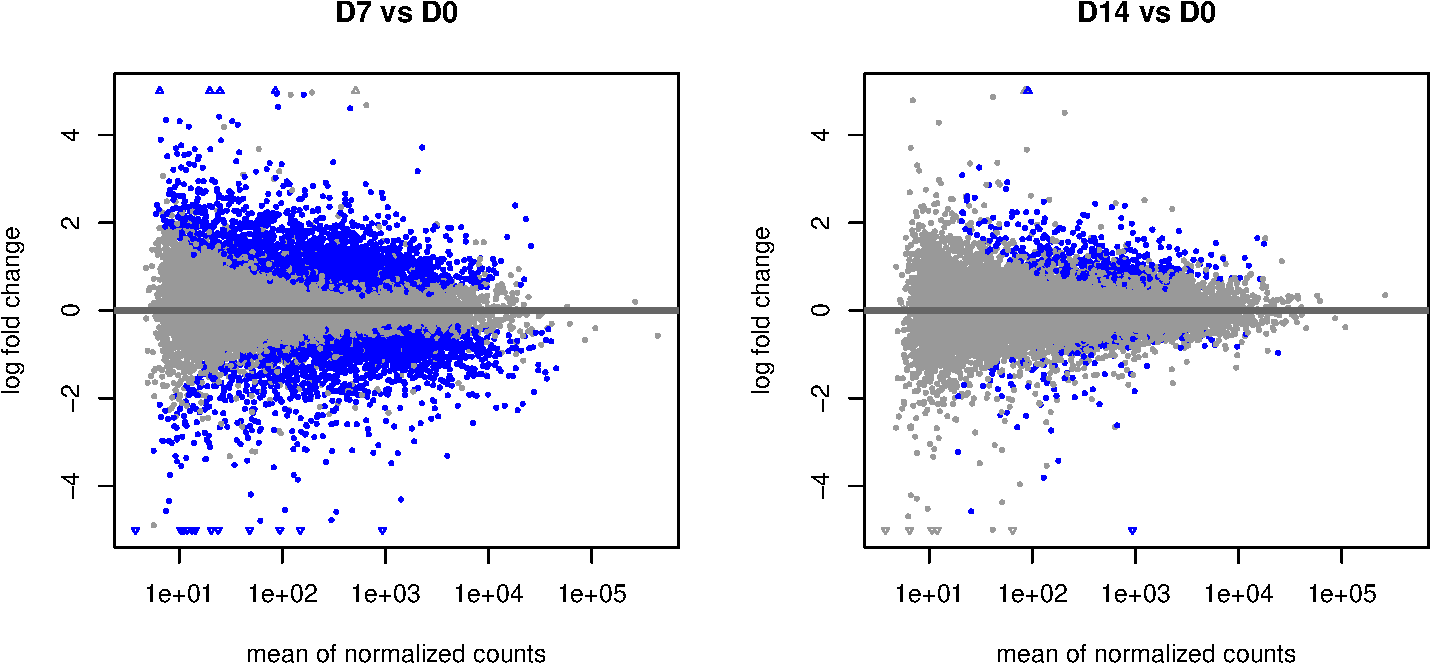
\includegraphics[keepaspectratio]{DESeq2_RNAseq_tutorial_files/figure-latex/ma-plots-1.pdf}}

\begin{Shaded}
\begin{Highlighting}[]
\FunctionTok{par}\NormalTok{(}\AttributeTok{mfrow =} \FunctionTok{c}\NormalTok{(}\DecValTok{1}\NormalTok{, }\DecValTok{1}\NormalTok{))}
\end{Highlighting}
\end{Shaded}

\subsubsection{How to interpret MA
plots}\label{how-to-interpret-ma-plots}

\begin{itemize}
\tightlist
\item
  \textbf{X-axis (A):} Mean expression level --- genes on the right are
  more highly expressed.
\item
  \textbf{Y-axis (M):} log₂ fold change --- above 0 means upregulated,
  below 0 means downregulated.
\item
  \textbf{Blue/red points:} Statistically significant DEGs (padj
  \textless{} 0.1 by default).
\item
  \textbf{What to look for:} The cloud of grey points should be centered
  around M = 0 (most genes don't change). If the whole cloud is shifted
  up or down, there may be a normalisation issue. You'll notice that
  low-expression genes (left side) have more scatter --- this is
  expected, since estimates are noisier with fewer counts. DESeq2's
  shrinkage estimator pulls extreme fold changes at low counts toward
  zero.
\end{itemize}

\begin{center}\rule{0.5\linewidth}{0.5pt}\end{center}

\subsection{Volcano Plots}\label{volcano-plots}

Volcano plots combine fold change and statistical significance in one
view, making it easy to see the most biologically meaningful DEGs.

\begin{Shaded}
\begin{Highlighting}[]
\CommentTok{\# Helper function: convert DESeq2 results to a tidy data frame}
\NormalTok{prep\_volcano }\OtherTok{\textless{}{-}} \ControlFlowTok{function}\NormalTok{(res, contrast\_label) \{}
  \FunctionTok{as.data.frame}\NormalTok{(res) }\SpecialCharTok{\%\textgreater{}\%}
    \FunctionTok{rownames\_to\_column}\NormalTok{(}\StringTok{"gene"}\NormalTok{) }\SpecialCharTok{\%\textgreater{}\%}
    \FunctionTok{filter}\NormalTok{(}\SpecialCharTok{!}\FunctionTok{is.na}\NormalTok{(padj)) }\SpecialCharTok{\%\textgreater{}\%}      \CommentTok{\# remove genes excluded from testing}
    \FunctionTok{mutate}\NormalTok{(}
      \AttributeTok{contrast =}\NormalTok{ contrast\_label,}
      \AttributeTok{sig =} \FunctionTok{case\_when}\NormalTok{(}
\NormalTok{        padj }\SpecialCharTok{\textless{}} \FloatTok{0.05} \SpecialCharTok{\&}\NormalTok{ log2FoldChange }\SpecialCharTok{\textgreater{}}  \DecValTok{1} \SpecialCharTok{\textasciitilde{}} \StringTok{"Up"}\NormalTok{,}
\NormalTok{        padj }\SpecialCharTok{\textless{}} \FloatTok{0.05} \SpecialCharTok{\&}\NormalTok{ log2FoldChange }\SpecialCharTok{\textless{}} \SpecialCharTok{{-}}\DecValTok{1} \SpecialCharTok{\textasciitilde{}} \StringTok{"Down"}\NormalTok{,}
        \ConstantTok{TRUE} \SpecialCharTok{\textasciitilde{}} \StringTok{"NS"}   \CommentTok{\# Not Significant}
\NormalTok{      )}
\NormalTok{    )}
\NormalTok{\}}

\NormalTok{volcano\_data }\OtherTok{\textless{}{-}} \FunctionTok{bind\_rows}\NormalTok{(}
  \FunctionTok{prep\_volcano}\NormalTok{(res\_D7\_vs\_D0,  }\StringTok{"D7 vs D0"}\NormalTok{),}
  \FunctionTok{prep\_volcano}\NormalTok{(res\_D14\_vs\_D0, }\StringTok{"D14 vs D0"}\NormalTok{)}
\NormalTok{)}
\end{Highlighting}
\end{Shaded}

\begin{Shaded}
\begin{Highlighting}[]
\NormalTok{volcanoPlot }\OtherTok{\textless{}{-}} \FunctionTok{ggplot}\NormalTok{(volcano\_data, }\FunctionTok{aes}\NormalTok{(}\AttributeTok{x =}\NormalTok{ log2FoldChange, }\AttributeTok{y =} \SpecialCharTok{{-}}\FunctionTok{log10}\NormalTok{(padj), }\AttributeTok{color =}\NormalTok{ sig)) }\SpecialCharTok{+}
  \FunctionTok{geom\_point}\NormalTok{(}\AttributeTok{alpha =} \FloatTok{0.5}\NormalTok{, }\AttributeTok{size =} \DecValTok{1}\NormalTok{) }\SpecialCharTok{+}
  \FunctionTok{scale\_color\_manual}\NormalTok{(}\AttributeTok{values =} \FunctionTok{c}\NormalTok{(}\StringTok{"Up"} \OtherTok{=} \StringTok{"red"}\NormalTok{, }\StringTok{"Down"} \OtherTok{=} \StringTok{"blue"}\NormalTok{, }\StringTok{"NS"} \OtherTok{=} \StringTok{"grey70"}\NormalTok{)) }\SpecialCharTok{+}
  \FunctionTok{geom\_vline}\NormalTok{(}\AttributeTok{xintercept =} \FunctionTok{c}\NormalTok{(}\SpecialCharTok{{-}}\DecValTok{1}\NormalTok{, }\DecValTok{1}\NormalTok{), }\AttributeTok{linetype =} \StringTok{"dashed"}\NormalTok{, }\AttributeTok{color =} \StringTok{"black"}\NormalTok{) }\SpecialCharTok{+}
  \FunctionTok{geom\_hline}\NormalTok{(}\AttributeTok{yintercept =} \SpecialCharTok{{-}}\FunctionTok{log10}\NormalTok{(}\FloatTok{0.05}\NormalTok{), }\AttributeTok{linetype =} \StringTok{"dashed"}\NormalTok{, }\AttributeTok{color =} \StringTok{"black"}\NormalTok{) }\SpecialCharTok{+}
  \FunctionTok{facet\_wrap}\NormalTok{(}\SpecialCharTok{\textasciitilde{}}\NormalTok{ contrast) }\SpecialCharTok{+}
  \FunctionTok{labs}\NormalTok{(}
    \AttributeTok{x     =} \StringTok{"log2 Fold Change"}\NormalTok{,}
    \AttributeTok{y     =} \StringTok{"{-}log10 adjusted p{-}value"}\NormalTok{,}
    \AttributeTok{color =} \StringTok{"Direction"}
\NormalTok{  ) }\SpecialCharTok{+}
  \FunctionTok{theme\_bw}\NormalTok{()}

\NormalTok{volcanoPlot}
\end{Highlighting}
\end{Shaded}

\pandocbounded{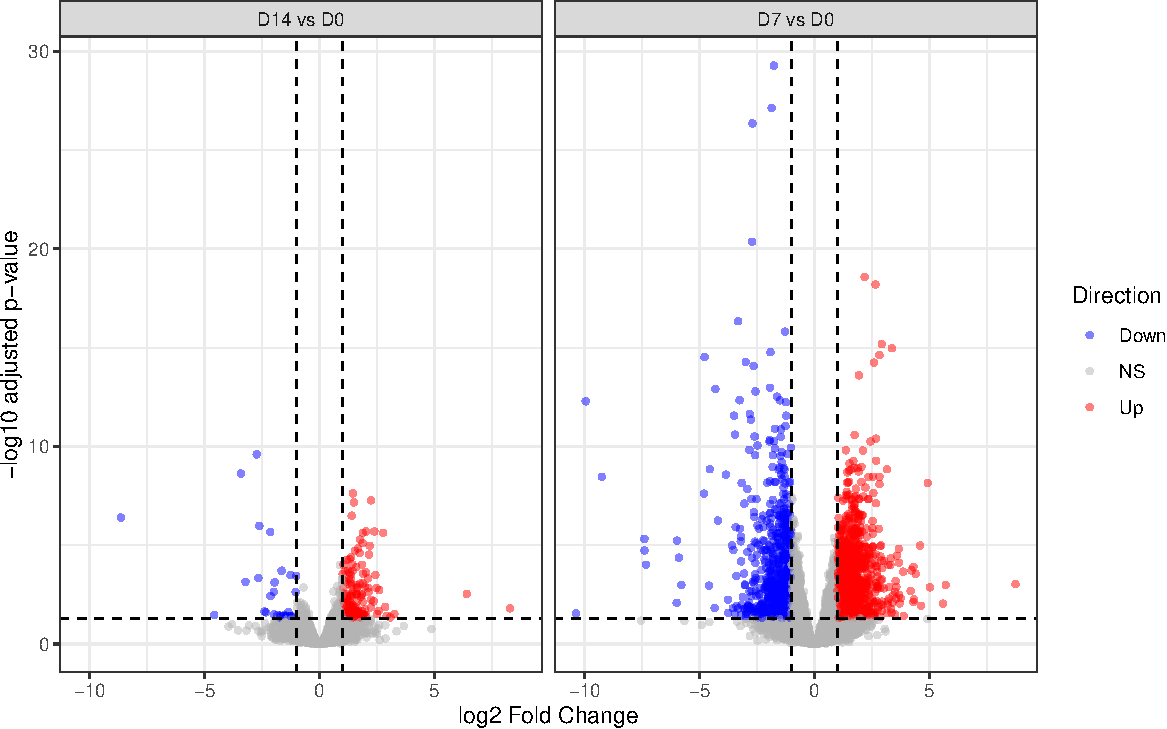
\includegraphics[keepaspectratio]{DESeq2_RNAseq_tutorial_files/figure-latex/volcano-plot-1.pdf}}

\begin{Shaded}
\begin{Highlighting}[]
\FunctionTok{ggsave}\NormalTok{(}\StringTok{"Volcano\_plot.pdf"}\NormalTok{, volcanoPlot, }\AttributeTok{device =} \StringTok{"pdf"}\NormalTok{)}
\end{Highlighting}
\end{Shaded}

\subsubsection{How to interpret volcano
plots}\label{how-to-interpret-volcano-plots}

\begin{itemize}
\tightlist
\item
  \textbf{X-axis:} Effect size. Right = upregulated in the later time
  point vs D0; left = downregulated.
\item
  \textbf{Y-axis:} Statistical confidence. Higher up = more significant
  (more negative log of padj).
\item
  \textbf{Dashed lines:} Our significance thresholds. The vertical lines
  mark \textbar log2FC\textbar{} = 1 (i.e., a 2-fold change); the
  horizontal line marks padj = 0.05.
\item
  \textbf{Coloured points (upper corners):} These are our ``hits'' ---
  genes that are both statistically significant AND biologically
  meaningful in magnitude. A gene can be statistically significant but
  have a tiny fold change (meaningful only with enormous sample sizes),
  or have a large fold change but high variability (not significant).
  The top corners capture both.
\item
  \textbf{Comparing panels:} More dots in the upper corners for D14 vs
  D0 than D7 vs D0 suggests the transcriptome changes accumulate over
  time --- a common finding in time-course experiments.
\end{itemize}

\begin{center}\rule{0.5\linewidth}{0.5pt}\end{center}

\subsection{Heatmap}\label{heatmap}

The heatmap lets us visualise the expression pattern of the top DEGs
across all samples at once, and see whether genes cluster into coherent
groups (e.g., early-response genes vs late-response genes).

\begin{Shaded}
\begin{Highlighting}[]
\CommentTok{\# Pool both contrasts, sort by padj, take the top 50 unique genes}
\NormalTok{top\_genes }\OtherTok{\textless{}{-}} \FunctionTok{bind\_rows}\NormalTok{(}
  \FunctionTok{as.data.frame}\NormalTok{(res\_D7\_vs\_D0)  }\SpecialCharTok{\%\textgreater{}\%} \FunctionTok{rownames\_to\_column}\NormalTok{(}\StringTok{"gene"}\NormalTok{),}
  \FunctionTok{as.data.frame}\NormalTok{(res\_D14\_vs\_D0) }\SpecialCharTok{\%\textgreater{}\%} \FunctionTok{rownames\_to\_column}\NormalTok{(}\StringTok{"gene"}\NormalTok{)}
\NormalTok{) }\SpecialCharTok{\%\textgreater{}\%}
  \FunctionTok{filter}\NormalTok{(}\SpecialCharTok{!}\FunctionTok{is.na}\NormalTok{(padj)) }\SpecialCharTok{\%\textgreater{}\%}
  \FunctionTok{arrange}\NormalTok{(padj) }\SpecialCharTok{\%\textgreater{}\%}
  \FunctionTok{distinct}\NormalTok{(gene, }\AttributeTok{.keep\_all =} \ConstantTok{TRUE}\NormalTok{) }\SpecialCharTok{\%\textgreater{}\%}   \CommentTok{\# keep each gene only once}
  \FunctionTok{slice\_head}\NormalTok{(}\AttributeTok{n =} \DecValTok{50}\NormalTok{) }\SpecialCharTok{\%\textgreater{}\%}
  \FunctionTok{pull}\NormalTok{(gene)}

\CommentTok{\# Extract VST{-}normalised counts for those genes}
\NormalTok{mat        }\OtherTok{\textless{}{-}} \FunctionTok{assay}\NormalTok{(vsd)[top\_genes, ]}

\CommentTok{\# Z{-}score each row (gene) so colours reflect relative change, not absolute expression}
\NormalTok{mat\_scaled }\OtherTok{\textless{}{-}} \FunctionTok{t}\NormalTok{(}\FunctionTok{scale}\NormalTok{(}\FunctionTok{t}\NormalTok{(mat)))}

\CommentTok{\# Column annotations}
\NormalTok{annotation\_col }\OtherTok{\textless{}{-}} \FunctionTok{data.frame}\NormalTok{(}\AttributeTok{Day =}\NormalTok{ pheno\_data}\SpecialCharTok{$}\NormalTok{Day)}
\FunctionTok{rownames}\NormalTok{(annotation\_col) }\OtherTok{\textless{}{-}} \FunctionTok{rownames}\NormalTok{(pheno\_data)}
\end{Highlighting}
\end{Shaded}

\begin{Shaded}
\begin{Highlighting}[]
\FunctionTok{pheatmap}\NormalTok{(}
\NormalTok{  mat\_scaled,}
  \AttributeTok{annotation\_col =}\NormalTok{ annotation\_col,}
  \AttributeTok{cluster\_rows   =} \ConstantTok{TRUE}\NormalTok{,}
  \AttributeTok{cluster\_cols   =} \ConstantTok{TRUE}\NormalTok{,}
  \AttributeTok{show\_rownames  =} \ConstantTok{TRUE}\NormalTok{,}
  \AttributeTok{show\_colnames  =} \ConstantTok{TRUE}\NormalTok{,}
  \AttributeTok{fontsize\_row   =} \DecValTok{7}\NormalTok{,}
  \AttributeTok{main           =} \StringTok{"Top 50 DEGs (scaled VST counts)"}
\NormalTok{)}
\end{Highlighting}
\end{Shaded}

\pandocbounded{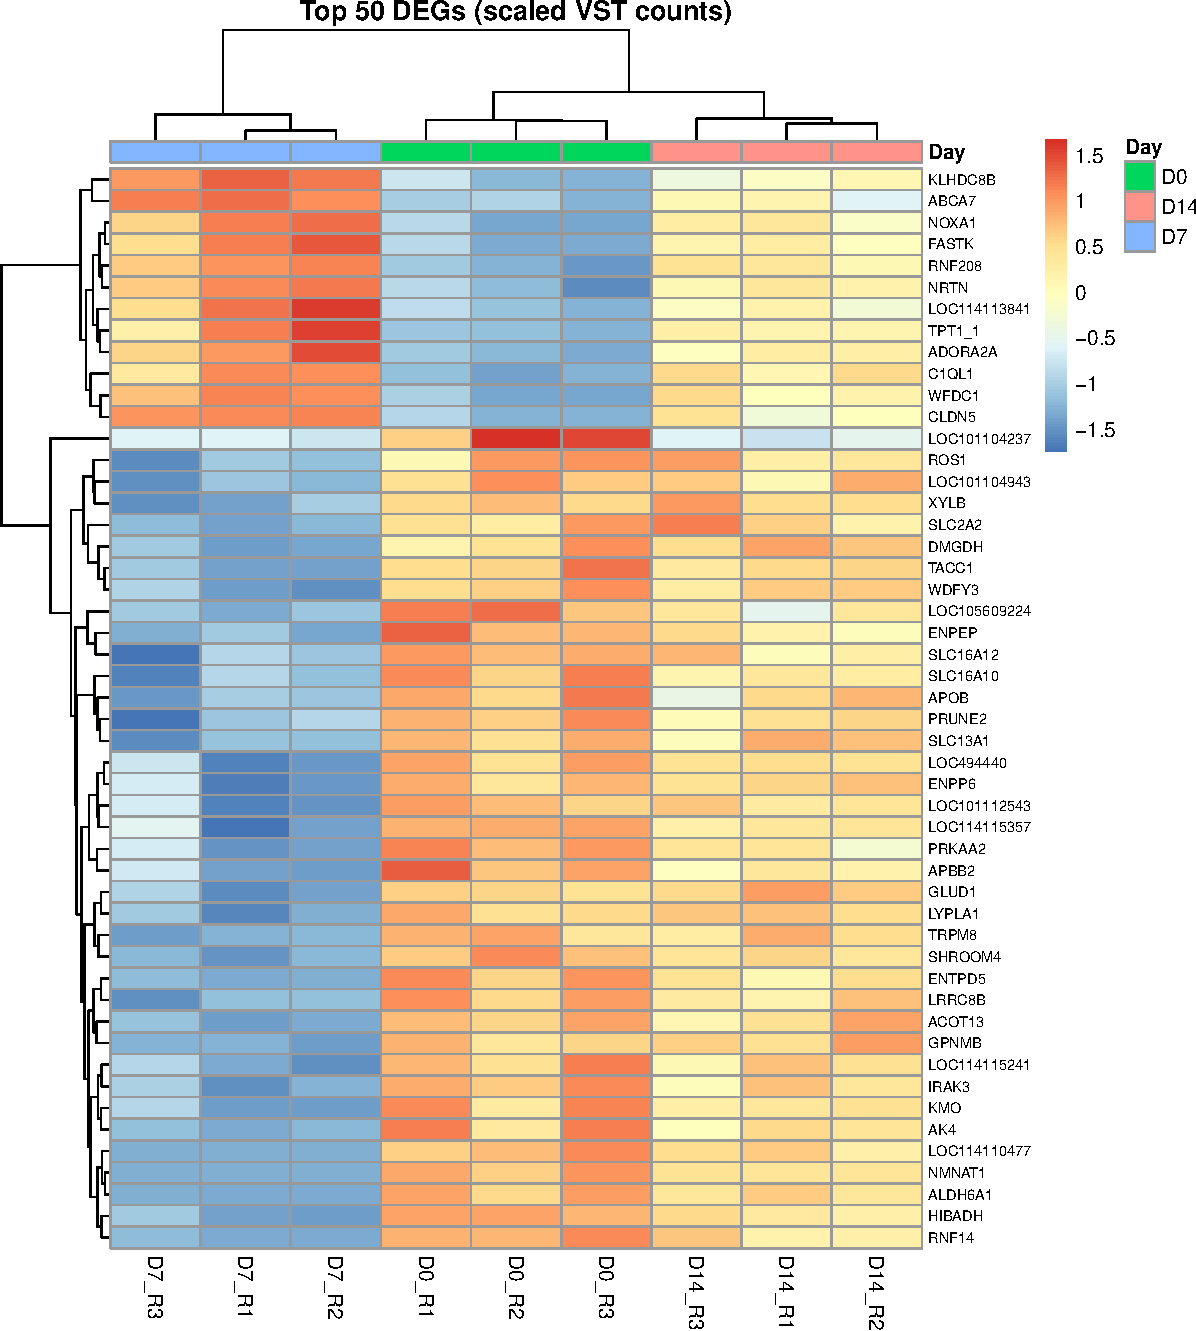
\includegraphics[keepaspectratio]{DESeq2_RNAseq_tutorial_files/figure-latex/heatmap-1.pdf}}

\subsubsection{How to interpret the
heatmap}\label{how-to-interpret-the-heatmap}

\begin{itemize}
\tightlist
\item
  \textbf{Colour:} Each cell's colour reflects the \textbf{z-score} of
  that gene in that sample. Blue = below the gene's mean expression; red
  = above the gene's mean. We z-score so that all genes are on the same
  scale regardless of their absolute expression level.
\item
  \textbf{Row clustering (genes):} Genes with similar expression
  patterns across samples are grouped together by hierarchical
  clustering. Look for distinct blocks --- e.g., a cluster that goes red
  at D14 but stays blue at D0 and D7 represents late-induced genes.
\item
  \textbf{Column clustering (samples):} Samples with similar overall
  expression profiles cluster together. Ideally, replicates of the same
  Day group next to each other, confirming biological reproducibility.
\item
  \textbf{Why pool contrasts for top genes?} Taking the 50 lowest padj
  genes from either comparison gives a more complete picture of the
  biology than looking at one contrast alone --- you'll catch genes that
  are most changed early (D7) or late (D14).
\end{itemize}

\begin{center}\rule{0.5\linewidth}{0.5pt}\end{center}

\section{Summary}\label{summary}

Here is a brief recap of the full workflow:

\begin{verbatim}
Raw count matrix
      │
      ▼
DESeqDataSetFromMatrix()   ← attach metadata & design
      │
      ▼
Filter low-count genes     ← remove noise, reduce multiple testing
      │
      ▼
DESeq()                    ← normalise → estimate dispersion → fit GLM → test
      │
      ├──── vst() → PCA          (QC: do samples separate as expected?)
      │
      ├──── results() → MA plot  (global view of effect size vs expression)
      │
      ├──── results() → Volcano  (which genes are significant AND large change?)
      │
      └──── results() → Heatmap  (patterns across top DEGs and all samples)
\end{verbatim}

\subsubsection{Key thresholds used in this
analysis}\label{key-thresholds-used-in-this-analysis}

\begin{longtable}[]{@{}
  >{\raggedright\arraybackslash}p{(\linewidth - 4\tabcolsep) * \real{0.5682}}
  >{\raggedright\arraybackslash}p{(\linewidth - 4\tabcolsep) * \real{0.1818}}
  >{\raggedright\arraybackslash}p{(\linewidth - 4\tabcolsep) * \real{0.2500}}@{}}
\toprule\noalign{}
\begin{minipage}[b]{\linewidth}\raggedright
Threshold
\end{minipage} & \begin{minipage}[b]{\linewidth}\raggedright
Value
\end{minipage} & \begin{minipage}[b]{\linewidth}\raggedright
Rationale
\end{minipage} \\
\midrule\noalign{}
\endhead
\bottomrule\noalign{}
\endlastfoot
Minimum counts filter & ≥ 10 counts in ≥ 3 samples & Remove unreliably
low-count genes \\
Adjusted p-value cutoff & \textless{} 0.05 & 5\% FDR \\
Fold-change cutoff & \textbar log2FC\textbar{} \textgreater{} 1 & At
least a 2-fold change \\
\end{longtable}

\begin{center}\rule{0.5\linewidth}{0.5pt}\end{center}

\section{Session Info}\label{session-info}

\begin{Shaded}
\begin{Highlighting}[]
\FunctionTok{sessionInfo}\NormalTok{()}
\end{Highlighting}
\end{Shaded}

\begin{verbatim}
## R version 4.5.1 (2025-06-13)
## Platform: aarch64-apple-darwin20
## Running under: macOS Sequoia 15.6
## 
## Matrix products: default
## BLAS:   /Library/Frameworks/R.framework/Versions/4.5-arm64/Resources/lib/libRblas.0.dylib 
## LAPACK: /Library/Frameworks/R.framework/Versions/4.5-arm64/Resources/lib/libRlapack.dylib;  LAPACK version 3.12.1
## 
## locale:
## [1] en_US.UTF-8/en_US.UTF-8/en_US.UTF-8/C/en_US.UTF-8/en_US.UTF-8
## 
## time zone: America/New_York
## tzcode source: internal
## 
## attached base packages:
## [1] stats4    stats     graphics  grDevices utils     datasets  methods  
## [8] base     
## 
## other attached packages:
##  [1] pheatmap_1.0.13             lubridate_1.9.4            
##  [3] forcats_1.0.0               stringr_1.5.2              
##  [5] dplyr_1.1.4                 purrr_1.1.0                
##  [7] readr_2.1.5                 tidyr_1.3.1                
##  [9] tibble_3.3.0                ggplot2_4.0.0              
## [11] tidyverse_2.0.0             DESeq2_1.50.2              
## [13] SummarizedExperiment_1.40.0 Biobase_2.70.0             
## [15] MatrixGenerics_1.22.0       matrixStats_1.5.0          
## [17] GenomicRanges_1.62.1        Seqinfo_1.0.0              
## [19] IRanges_2.44.0              S4Vectors_0.48.1           
## [21] BiocGenerics_0.56.0         generics_0.1.4             
## 
## loaded via a namespace (and not attached):
##  [1] gtable_0.3.6        xfun_0.53           lattice_0.22-7     
##  [4] tzdb_0.5.0          vctrs_0.6.5         tools_4.5.1        
##  [7] parallel_4.5.1      pkgconfig_2.0.3     Matrix_1.7-3       
## [10] RColorBrewer_1.1-3  S7_0.2.0            lifecycle_1.0.4    
## [13] compiler_4.5.1      farver_2.1.2        textshaping_1.0.3  
## [16] tinytex_0.57        codetools_0.2-20    htmltools_0.5.8.1  
## [19] yaml_2.3.10         pillar_1.11.0       BiocParallel_1.44.0
## [22] DelayedArray_0.36.1 abind_1.4-8         tidyselect_1.2.1   
## [25] locfit_1.5-9.12     digest_0.6.37       stringi_1.8.7      
## [28] labeling_0.4.3      fastmap_1.2.0       grid_4.5.1         
## [31] cli_3.6.5           SparseArray_1.10.10 magrittr_2.0.4     
## [34] S4Arrays_1.10.1     dichromat_2.0-0.1   withr_3.0.2        
## [37] scales_1.4.0        timechange_0.3.0    rmarkdown_2.29     
## [40] XVector_0.50.0      ragg_1.5.0          hms_1.1.3          
## [43] evaluate_1.0.5      knitr_1.50          rlang_1.1.6        
## [46] Rcpp_1.1.0          glue_1.8.0          rstudioapi_0.17.1  
## [49] R6_2.6.1            systemfonts_1.2.3
\end{verbatim}

\end{document}
